\documentclass[a4paper, 11pt]{article}
\usepackage{amsmath}
\usepackage{graphicx}
\usepackage{geometry}
\usepackage{listings}
\usepackage{xcolor}
\usepackage{bm}
\usepackage{caption,subcaption}
\geometry{scale=0.8}
\linespread{1.5}
\usepackage[colorlinks,linkcolor=red,anchorcolor=blue]{hyperref}
\usepackage{listings}
\usepackage{enumitem}
\usepackage{algorithm}
\usepackage{algorithmicx}
\usepackage{algpseudocode}


\lstset{
language={Python},
frame=shadowbox,
breaklines=true,
 numbers=left,
 backgroundcolor=\color[RGB]{245,245,244},
 rulesepcolor=\color{red!20!green!20!blue!20},
 numberstyle={\color[RGB]{0,192,192}\tiny},
 basicstyle=\footnotesize
 }
\setenumerate[1]{itemsep=0pt,partopsep=0pt,parsep=\parskip,topsep=0pt}
\setitemize[1]{itemsep=0pt,partopsep=0pt,parsep=\parskip,topsep=0pt}
\setdescription{itemsep=0pt,partopsep=0pt,parsep=\parskip,topsep=0pt}


\title{	
\normalfont \normalsize
\textsc{School of Data and Computer Science, Sun Yat-sen University} \\ [25pt] %textsc small capital letters
\rule{\textwidth}{0.5pt} \\[0.4cm] % Thin top horizontal rule
\huge  E16 Deep Q-Learning (C++/Python)\\ % The assignment title
\rule{\textwidth}{2pt} \\[0.5cm] % Thick bottom horizontal rule
\author{16110917 Zhaoshuai Liu}
\date{\normalsize\today}
}

\begin{document}
\maketitle
\tableofcontents
\newpage


\section{Introduction to Reinforcement Learning}

{\color{blue}{\textbf{English version}: \href{https://blog.algorithmia.com/introduction-to-reinforcement-learning/}{Introduction to Reinforcement Learning}\\
\textbf{Chinese version}: \url{https://blog.csdn.net/qq_28168421/article/details/81784563}}}

We only understand a sliver of how the brain works, but we \emph{do}
know that it often learns through trial and error. We're rewarded when
we do good things and punished when we do the wrong ones; that's how we
figure out how to live. Reinforcement Learning puts computational power
behind that exact process and lets us model it with software.

\subsection{\textbf{What Is Reinforcement Learning?}}

The easiest mental model to aid in understanding Reinforcement Learning
(RL) is as a video game, which coincidentally is
\href{https://www.cs.toronto.edu/~vmnih/docs/dqn.pdf}{one of the most
popular applications} of RL algorithms. In a typical video game, you
might have:

\begin{itemize}
\itemsep1pt\parskip0pt\parsep0pt
\item
  An \textbf{agent} (the player) who moves around doing stuff
\item
  An \textbf{action} that the agent takes (moves upward one space, sells
  cloak)
\item
  A \textbf{reward} that the agent acquires (coins, killing other
  players, etc.)
\item
  An \textbf{environment} that the agent exists in (a map, a room)
\item
  A \textbf{state} that the agent currently exists in (on a particular
  square of a map, part of a room)
\item
  A \textbf{goal} of your agent getting as many rewards as possible
\end{itemize}

These literally are the exact building blocks of Reinforcement Learning
(maybe Machine Learning is just a game?). In RL, we guide an
\textbf{agent} through an \textbf{environment}, \textbf{state} by
\textbf{state}, by issuing a \textbf{reward} every time the agent does
the right thing. If you've heard the term
\href{https://en.wikipedia.org/wiki/Markov_decision_process}{Markov
Decision Process} thrown around, it pretty much describes this exact
setting.

For a visual aid, you can think of a mouse in a maze:

\includegraphics[width=0.65\textwidth]{Pic/word-image-3.png}

Source:
\href{https://medium.com/machine-learning-for-humans/reinforcement-learning-6eacf258b265}{Machine
Learning for Humans}

If you were navigating the maze yourself and your goal was to collect as
many rewards as possible (the water droplets and cheese), what would you
do? At each \textbf{state} (position in the maze), you'd calculate what
steps you need to take to reach the rewards near you. If there are 3
rewards on your right and 1 on your left, you'd go right.

This is how Reinforcement Learning works. At each state, the agent makes
an educated calculation about all of the possible \textbf{actions}
(left, right, up, down, you name it) and takes the action that'll yield
the best result. After completing this process a few times, you'd
imagine that our mouse might know the maze pretty well.

But how exactly do you decide what the ``best result'' is?

\subsection{\textbf{Decision Making in Reinforcement Learning}}

There are 2 broad approaches for how you can teach your agent to make
the right decisions in a Reinforcement Learning environment.

\subparagraph{\emph{Policy Learning}}

Policy learning is best understood as a set of very detailed directions
-- it tells the agent exactly what to do at each state. A part of a
policy might look something like: ``if you approach an enemy and the
enemy is stronger than you, turn backwards.'' If you think of a policy
as a function, it only has one input: the state. But knowing in advance
what your policy should be isn't easy, and requires deep knowledge of
the complex function that maps state to goal.

There's been some very interesting research in applying Deep Learning to
learn policies for Reinforcement Learning scenarios.
\href{http://karpathy.github.io/2016/05/31/rl/}{Andrej Karpathy
implemented a neural net} to teach an agent how to play the classic game
of pong. This shouldn't surprise us, since neural nets can be very good
at approximating complicated functions.

\subparagraph{\emph{Q-Learning / Value Functions}}

Another way of guiding our agent is not by explicitly telling her what
to do at each point, but by giving her \textbf{a framework} to make her
own decisions. Unlike policy learning, Q-Learning takes \emph{two
inputs} -- state \emph{and} action -- and returns a value for each pair.
If you're at an intersection, Q-learning will tell you the expected
value of each action your agent could take (left, right, etc.).

One of the quirks of Q-Learning is that it doesn't just estimate the
\emph{immediate} value of taking an action in a given state: it also
adds in all of the potential future value that could be had if you take
the specified action. For readers familiar with corporate finance,
Q-Learning is sort of like a discounted cash flow analysis -- it takes
all potential future value into account when determining the current
value of an action (or asset). In fact, Q-Learning even uses a
\emph{discount-factor} to model the fact that rewards in the future are
worth less than rewards now.

Policy Learning and Q-Learning are the two mainstays of how to guide an
agent in Reinforcement Learning, but a bunch of new approaches have been
using Deep Learning to combine the two or attempt other creative
solutions. DeepMind published
\href{https://storage.googleapis.com/deepmind-media/dqn/DQNNaturePaper.pdf}{a
paper about using neural nets (called Deep Q Networks)} to approximate
Q-Learning functions, and achieved impressive results. A few years
later, they pioneered
\href{https://medium.com/emergent-future/simple-reinforcement-learning-with-tensorflow-part-8-asynchronous-actor-critic-agents-a3c-c88f72a5e9f2}{a
method called A3C} that combined Q-Learning and Policy Learning
approaches.

Adding neural nets into anything can make it sound complicated. Just
remember that all of these learning approaches have a simple goal: to
effectively guide your agent through the environment and acquire the
most rewards. That's it.

\subsection{\textbf{Practical Applications of Reinforcement
Learning}}

While the concepts supporting Reinforcement Learning have been around
for decades, unfortunately
\href{https://www.oreilly.com/ideas/practical-applications-of-reinforcement-learning-in-industry}{it's
rarely implemented in practice today in business contexts}. There are a
number of reasons for that (see the challenges section below), but they
all follow a similar thread: Reinforcement Learning struggles to
efficiently beat out other algorithms for well defined tasks.

Most of the practical application of Reinforcement Learning in the past
decade has been in the realm of video games. Cutting edge Reinforcement
Learning algorithms have achieved impressive results in classic and
modern games, often beating out their human counterparts by a
significant margin.

This graph is from the above mentioned DQN paper by DeepMind. For more
than half the games tested, their agent was able to outperform human
benchmarks, often by more than double the skill level. For certain games
though, their algorithms weren't even close to human performance.

The other major area where RL has seen some practical success is in
\href{https://vmayoral.github.io/robots,/ai,/deep/learning,/rl,/reinforcement/learning/2016/07/06/rl-intro/}{robotics
and industrial automation}. Robots can easily be understood as agents in
an environment, and Reinforcement Learning has been shown to be
\href{https://www.youtube.com/watch?v=ZhsEKTo7V04}{a feasible teaching
solution}.
\href{https://environment.google/projects/machine-learning/}{Google has
also made progress using Reinforcement Learning} to cut down costs in
their data centers.

\href{https://mlhc17mit.github.io/slides/lecture13.pdf}{Healthcare} and
\href{http://pact.cs.cmu.edu/pubs/New\%20potentials\%20for\%20ITS-source.pdf}{education}
are also promising areas for Reinforcement Learning, but most of the
work is purely academic at this point.

\includegraphics[width=\textwidth]{Pic/word-image-4.png}



\begin{center}\rule{6in}{0.4pt}\end{center}

\subsection{\textbf{Challenges With Implementing Reinforcement
Learning}}

While extremely promising,
\href{https://www.alexirpan.com/2018/02/14/rl-hard.html}{Reinforcement
Learning is notoriously difficult to implement} in practice.

\includegraphics[width=0.95\textwidth]{Pic/word-image-5.png}

Source: \href{https://www.alexirpan.com/2018/02/14/rl-hard.html}{Alex
Irpan}

The first issue is data: Reinforcement Learning typically requires a
\emph{ton} of training data to reach accuracy levels that other
algorithms can get to more efficiently. RainbowDQN (from the most recent
DeepMind paper) requires 18 Million frames of Atari gameplay to train
properly, or about 83 hours of play time. A human can pick up the game
\emph{much}faster than that. This issue seems to hold across disciplines
(\href{https://youtu.be/hx_bgoTF7bs}{like learning a running gait}).

Another challenge in implementing Reinforcement Learning is the
domain-specificity problem. Reinforcement Learning is a general
algorithm, in that it should theoretically work for all different types
of problems. But most of those problems have a domain-specific solution
that will work better than RL, like
\href{https://homes.cs.washington.edu/~todorov/papers/TassaIROS12.pdf}{online
trajectory optimization for MuJuCo robots}. There's always a tradeoff
between scope and intensity.

Finally, the most pressing issue with Reinforcement Learning as it
currently stands is the design of the reward function (recall Q-Learning
and Policy Learning). If the algorithm designers are the ones setting up
rewards, then model results are extremely subjective to the bias of the
designers. Even when set up properly, Reinforcement Learning has this
clever way of
\href{https://www.alexirpan.com/public/rl-hard/upsidedown_half_cheetah.mp4}{finding
ways around what you want it to do} and getting stuck in local optima.

With so much cutting edge research focused on advancing Reinforcement
Learning, expect some of these kinks to get ironed out over time.

\subsection{\textbf{\color{orange}{Resources}}}

\subparagraph{\textbf{Frameworks and Packages}}

\href{http://glue.rl-community.org/wiki/Main_Page}{RL-Glue} --
``\emph{RL-Glue (Reinforcement Learning Glue) provides a standard
interface that allows you to connect}\emph{reinforcement
learning}\emph{agents, environments, and experiment programs together,
even if they are written in different languages.}''

\href{https://gym.openai.com/}{Gym} (OpenAI) -- ``\emph{Gym is a toolkit
for developing and comparing reinforcement learning algorithms. It
supports teaching agents everything from}\emph{walking}\emph{to playing
games like}\emph{Pong~}\emph{or}\emph{Pinball}\emph{.}''

\href{https://github.com/deeplearning4j/rl4j}{RL4J} (DL4J) --
``\emph{RL4J is a reinforcement learning framework integrated with
deeplearning4j and released under an Apache 2.0 open-source license.}''

\href{https://github.com/reinforceio/tensorforce}{TensorForce}
(Reinforce.io) -- ``\emph{A TensorFlow library for applied reinforcement
learning.}''

\subparagraph{\textbf{Reading}}

\href{https://medium.com/machine-learning-for-humans/reinforcement-learning-6eacf258b265}{Machine
Learning for Humans, Part 5: Reinforcement Learning} (Machine Learning
for Humans) -- ``\emph{In reinforcement learning (RL) there's no answer
key, but your reinforcement learning agent still has to decide how to
act to perform its task. In the absence of existing training data, the
agent learns from experience. It collects the training examples (``this
action was good, that action was bad'') through trial-and-error as it
attempts its task, with the goal of maximizing long-term reward.}''

\href{https://medium.freecodecamp.org/an-introduction-to-reinforcement-learning-4339519de419}{An
Introduction to Reinforcement Learning} (freeCodeCamp) --
``\emph{Reinforcement learning is an important type of Machine Learning
where an agent learn how to behave in a environment by performing
actions and seeing the results. In recent years, we've seen a lot of
improvements in this fascinating area of research. In this series of
articles, we will focus on learning the different architectures used
today to solve Reinforcement Learning problems.}''

\href{https://deeplearning4j.org/deepreinforcementlearning}{A Beginner's
Guide to Deep Reinforcement Learning} (DL4J) -- ``\emph{Reinforcement
learning refers to goal-oriented algorithms, which learn how to attain a
complex objective (goal) or maximize along a particular dimension over
many steps; for example, maximize the points won in a game over many
moves. They can start from a blank slate, and under the right conditions
they achieve superhuman performance. Like a child incentivized by
spankings and candy, these algorithms are penalized when they make the
wrong decisions and rewarded when they make the right ones -- this is
reinforcement.}''

\href{https://deepmind.com/blog/deep-reinforcement-learning/}{Deep
Reinforcement Learning} (DeepMind) -- ``\emph{Humans excel at solving a
wide variety of challenging problems, from low-level motor control
through to high-level cognitive tasks. Our goal at DeepMind is to create
artificial agents that can achieve a similar level of performance and
generality. Like a human, our agents learn for themselves to achieve
successful strategies that lead to the greatest long-term rewards.}''

\href{http://amid.fish/reproducing-deep-rl}{Lessons Learned Reproducing
a Deep Reinforcement Learning Paper} (Amid Fish) -- ``\emph{I've seen a
few recommendations that reproducing papers is a good way of levelling
up machine learning skills, and I decided this could be an interesting
one to try with. It was indeed a super fun project, and I'm happy to
have tackled it -- but looking back, I realise it wasn't exactly the
experience I thought it would be. If you're thinking about reproducing
papers too, here are some notes on what surprised me about working with
deep RL.}''

\subparagraph{\textbf{Papers}}

\href{https://arxiv.org/abs/1712.01815}{Mastering Chess and Shogi by
Self-Play with a General Reinforcement Learning Algorithm} (13 authors!)
-- ``\emph{In this paper, we generalise this approach into a single
AlphaZero algorithm that can achieve, tabula rasa, superhuman
performance in many challenging domains. Starting from random play, and
given no domain knowledge except the game rules, AlphaZero achieved
within 24 hours a superhuman level of play in the games of chess and
shogi (Japanese chess) as well as Go, and convincingly defeated a
world-champion program in each case.}''

\href{https://arxiv.org/abs/1701.07274}{Deep Reinforcement Learning: An
Overview} (Li) -- ``\emph{We give an overview of recent exciting
achievements of deep reinforcement learning (RL). We discuss six core
elements, six important mechanisms, and twelve applications. We start
with background of machine learning, deep learning and reinforcement
learning. Next we discuss core RL elements, including value function, in
particular, Deep Q-Network (DQN), policy, reward, model, planning, and
exploration.}''

\href{http://www.cl.cam.ac.uk/~ey204/teaching/ACS/R244_2017_2018/papers/mnih_nips_2013.pdf}{Playing
Atari with Deep Reinforcement Learning} (DeepMind) -- ``\emph{We present
the first deep learning model to successfully learn control policies
directly from high-dimensional sensory input using reinforcement
learning. The model is a convolutional neural network, trained with a
variant of Q-learning, whose input is raw pixels and whose output is a
value function estimating future rewards. We apply our method to seven
Atari 2600 games from the Arcade Learning Environment, with no
adjustment of the architecture or learning algorithm. We find that it
outperforms all previous approaches on six of the games and surpasses a
human expert on three of them.}''

\href{https://web.stanford.edu/class/psych209/Readings/MnihEtAlHassibis15NatureControlDeepRL.pdf}{Human-Level
Control Through Deep Reinforcement Learning} (DeepMind) -- ``\emph{The
theory of reinforcement learning provides a normative account, deeply
rooted in psychological and neuroscientific perspectives on animal
behaviour, of how agents may optimize their control of an environment.
To use reinforcement learning successfully in situations approaching
real-world complexity, however, agents are confronted with a difficult
task: they must derive efficient representations of the environment from
high-dimensional sensory inputs, and use these to generalize past
experience to new situations.}''

\subparagraph{\textbf{Lectures and Videos}}

\href{https://www.udacity.com/course/reinforcement-learning-{}-ud600}{Reinforcement
Learning} (Udacity, Georgia Tech) -- ``\emph{You should take this course
if you have an interest in machine learning and the desire to engage
with it from a theoretical perspective. Through a combination of classic
papers and more recent work, you will explore automated decision-making
from a computer-science perspective. You will examine efficient
algorithms, where they exist, for single-agent and multi-agent planning
as well as approaches to learning near-optimal decisions from
experience. At the end of the course, you will replicate a result from a
published paper in reinforcement learning.''}

\href{http://web.stanford.edu/class/cs234/index.html}{CS234:
Reinforcement Learning} (Stanford) --~''\emph{To realize the dreams and
impact of AI requires autonomous systems that learn to make good
decisions. Reinforcement learning is one powerful paradigm for doing so,
and it is relevant to an enormous range of tasks, including robotics,
game playing, consumer modeling and healthcare. This class will provide
a solid introduction to the field of reinforcement learning and students
will learn about the core challenges and approaches, including
generalization and exploration.}''

\href{http://rll.berkeley.edu/deeprlcourse/}{CS 294: Deep Reinforcement
Learning, Fall 2017} (Berkeley) -- ``\emph{This course will assume some
familiarity with reinforcement learning, numerical optimization and
machine learning. Students who are not familiar with the concepts below
are encouraged to brush up using the references provided right below
this list. We'll review this material in class, but it will be rather
cursory.''}

\href{https://www.udemy.com/deep-reinforcement-learning-in-python/}{Advanced
AI: Deep Reinforcement Learning in Python} (Udemy) -- ``\emph{This
course is all about the application of deep learning and neural networks
to reinforcement learning. If you've taken my first reinforcement
learning class, then you know that reinforcement learning is on the
bleeding edge of what we can do with AI. Specifically, the combination
of deep learning with reinforcement learning has led to AlphaGo beating
a world champion in the strategy game Go, it has led to self-driving
cars, and it has led to machines that can play video games at a
superhuman level.}''

\subparagraph{\textbf{Tutorials}}

\href{https://www.analyticsvidhya.com/blog/2017/01/introduction-to-reinforcement-learning-implementation/}{Simple
Beginner's}\href{https://www.analyticsvidhya.com/blog/2017/01/introduction-to-reinforcement-learning-implementation/}{G}\href{https://www.analyticsvidhya.com/blog/2017/01/introduction-to-reinforcement-learning-implementation/}{uide
to Reinforcement Learning
\&}\href{https://www.analyticsvidhya.com/blog/2017/01/introduction-to-reinforcement-learning-implementation/}{I}\href{https://www.analyticsvidhya.com/blog/2017/01/introduction-to-reinforcement-learning-implementation/}{ts}\href{https://www.analyticsvidhya.com/blog/2017/01/introduction-to-reinforcement-learning-implementation/}{I}\href{https://www.analyticsvidhya.com/blog/2017/01/introduction-to-reinforcement-learning-implementation/}{mplementation}
(Analytics Vidhya) -- ``\emph{Today, we will explore Reinforcement
Learning -- a goal-oriented learning based on interaction with
environment. Reinforcement Learning is said to be the hope of true
artificial intelligence. And it is rightly said so, because the
potential that Reinforcement Learning possesses is immense}.''

\href{https://medium.com/emergent-future/simple-reinforcement-learning-with-tensorflow-part-0-q-learning-with-tables-and-neural-networks-d195264329d0}{Simple
Reinforcement Learning with Tensorflow Part 0: Q-Learning with Tables
and Neural Networks} (Arthur Juliani) -- ``\emph{For this tutorial in my
Reinforcement Learning series, we are going to be exploring a family of
RL algorithms called Q-Learning algorithms. These are a little different
than the policy-based algorithms that will be looked at in the the
following tutorials (Parts 1--3). Instead of starting with a complex and
unwieldy deep neural network, we will begin by implementing a simple
lookup-table version of the algorithm, and then show how to implement a
neural-network equivalent using Tensorflow.}''

\href{https://web.mst.edu/~gosavia/tutorial.pdf}{A Tutorial for
Reinforcement Learning} (Abhijit Gosavi) -- ``\emph{The tutorial is
written for those who would like an introduction to reinforcement
learning (RL). The aim is to provide an intuitive presentation of the
ideas rather than concentrate on the deeper mathematics underlying the
topic.}''
\section{Q-learning vs SARSA}
\textbf{Q-learning} is an off-policy reinforcement learning algorithm. In Q-learning and related algorithms, an agent tries to learn the optimal policy from its history of interaction with the environment. 

We treat this history of interaction as a sequence of experiences, where an experience is a tuple $\langle s,a,r,s'\rangle$ which means that the agent was in state $s$, it did action a, it received reward r, and it went into state $s$. These experiences will be the data from which the
agent can learn what to do. As in decision-theoretic planning, the aim is for the agent to maximize its value, which is usually the discounted reward.

\includegraphics[width=0.8\textwidth]{Pic/qlearning}

Q-learning learns an optimal policy no matter what the agent does, as long as it explores enough. There may be cases where ignoring what the agent actually does is dangerous (there will be large negative rewards). An alternative is to learn the value of the policy the agent is actually carrying out so that it can be iteratively improved. As a result, the learner can take into account the costs associated with exploration.

An \textbf{off-policy} learner learns the value of the optimal policy independently of the agent’s actions. Q-learning is an off-policy learner. An on-policy learner
learns the value of the policy being carried out by the agent, including the exploration steps.

\textbf{SARSA} (so called because it uses state-action-reward-state-action experiences to update the Q-values) is an \textbf{on-policy} reinforcement learning algorithm that estimates the value of the policy being followed. An experience in SARSA is of the form $\langle s,a,r,s',a'\rangle$, which means that the agent was in state $s$, did action $a$, received reward $r$, and ended up in state $s$, from which it decided to do action $a$. This provides a new experience to update $Q(s, a)$. The new value that
this experience provides is $r+\gamma Q(s',a')$.

SARSA takes into account the current exploration policy which, for example, may be greedy with random steps. It can find a different policy than Qlearning in situations when exploring may incur large penalties. For example,
when a robot goes near the top of stairs, even if this is an optimal policy, it may be dangerous for exploration steps. SARSA will discover this and adopt a policy that keeps the robot away from the stairs. It will find a policy that is optimal, taking into account the exploration inherent in the policy.

\includegraphics[width=0.7\textwidth]{Pic/sarsa}
\section{Deep Q-Network (DQN) }
We consider tasks in which an agent interacts with an environment $\mathcal{E}$, in this case the Atari emulator, in a sequence of actions, observations and rewards. 
At each time-step the agent selects an action $a_t$ from the set of legal game actions, $\mathcal{A}=\{1, \ldots, K \}$. The action is passed to the emulator and modifies its internal state and the game score. In general $\mathcal{E}$ may be stochastic. The emulator's internal state is not observed by the agent,  instead it observes an image $x_t\in\mathbb{R}^d$ from the emulator, which is a vector of raw pixel values representing the current screen. In addition it receives a reward $r_t$ representing the change in game score. Note that in general the game score may depend on the whole prior sequence of actions and observations; feedback about an action may only be received after many thousands of time-steps have elapsed. 

Since the agent only observes images of the current screen, the task is partially observed and many emulator states are perceptually aliased, i.e. it is impossible to fully understand the current situation from only the current screen $x_t$. We therefore consider sequences of actions and observations, $s_t = {x_1, a_1, x_2, ..., a_{t-1}, x_t}$, and learn game strategies that depend upon these sequences. All sequences in the emulator are assumed to terminate in a finite number of time-steps. This formalism gives rise to a large but finite Markov decision process (MDP) in which each sequence is a distinct state. As a result, we can apply standard reinforcement learning methods for MDPs, simply by using the complete sequence $s_t$ as the state representation at time $t$.

The goal of the agent is to interact with the emulator by selecting actions in a way that maximises future rewards. We make the standard assumption that future rewards are discounted by a factor of $\gamma$ per time-step, and define the future discounted \emph{return} at time $t$ as $R_t = \sum_{t'=t}^{T} \gamma^{t'-t} r_{t'}$, where $T$
is the time-step at which the game terminates. We define the optimal action-value function $Q^*(s,a)$ as the maximum expected return achievable by following any strategy, after seeing some sequence $s$ and then taking some action $a$, $Q^*(s,a) = \max_{\pi} \mathbb E[R_t | s_t=s, a_t=a, \pi ]$, where $\pi$ is a policy mapping sequences to actions (or distributions over actions).

The optimal action-value function obeys an important identity known as the \emph{Bellman equation}. This is based on the following intuition: if the optimal value $Q^*(s',a')$ of the sequence $s'$ at the next time-step was known for all possible actions $a'$, then the optimal strategy is to select the action $a'$ maximising the expected value of $r + \gamma Q^*(s',a')$,
%
\begin{align}
Q^*(s,a) &= \mathbb E_{s' \sim \mathcal{E}}[r + \gamma \max_{a'} Q^*(s', a') \Big| s, a]
\end{align}
%
The basic idea behind many reinforcement learning algorithms is to estimate the action-value function, by using the Bellman equation as an iterative update, $Q_{i+1}(s,a) = \mathbb{E}\left[ r + \gamma \max_{a'} Q_i(s', a') | s, a \right]$. Such \emph{value iteration} algorithms converge to the optimal action-value function, $Q_i \rightarrow Q^*$ as $i \rightarrow \infty$. In practice, this basic approach is totally impractical, because the action-value function is estimated separately for each sequence, without any generalisation. Instead, it is common to use a function approximator to estimate the action-value function, $Q(s,a; \theta) \approx Q^*(s,a)$. In the reinforcement learning community this is typically a linear function approximator, but sometimes a non-linear function approximator is used instead, such as a neural network. We refer to a neural network function approximator with weights $\theta$ as a Q-network. A Q-network can be trained by minimising a sequence of loss functions $L_i(\theta_i)$ that changes at each iteration $i$,
%
\begin{align}
L_i\left(\theta_i\right) &= \mathbb E_{s,a \sim \rho(\cdot)}[\left(y_i - Q \left(s,a ; \theta_i \right) \right)^2],
\label{eq:q-learning-loss}
\end{align}
%
where $y_i = \mathbb E_{s' \sim \mathcal{E}}[r + \gamma \max_{a'} Q(s', a'; \theta_{i-1}) | s, a ]$ is the target for iteration $i$ and $\rho(s,a)$ is a probability distribution over sequences $s$ and actions $a$ that we refer to as the \emph{behaviour distribution}. The parameters from the previous iteration $\theta_{i-1}$ are held fixed when optimising the loss function $L_i\left(\theta_i\right)$. 
Note that the targets depend on the network weights; this is in contrast with the targets used for supervised learning, which are fixed before learning begins.
% This can lead to feedback effects and even divergence during training, which is a major reason why reinforcement learning is more challenging than supervised learning.
Differentiating the loss function with respect to the weights we arrive at the following gradient,
%
\begin{align}
\nabla_{\theta_i} L_i\left(\theta_i\right) &= \mathbb{E}_{s,a \sim \rho(\cdot); s' \sim \mathcal{E}} \left[ \left( r + \gamma \max_{a'} Q(s', a'; \theta_{i-1}) - Q(s,a ; \theta_i ) \right) \nabla_{\theta_i} Q(s,a;\theta_{i}) \right] .
\label{eq:q-learning-gradient}
\end{align}
%
Rather than computing the full expectations in the above gradient, it is often computationally expedient to optimise the loss function by stochastic gradient descent. If the weights are updated after every time-step, and the expectations are replaced by single samples from the behaviour distribution $\rho$ and the emulator $\mathcal{E}$ respectively, then we arrive at the familiar \emph{Q-learning} algorithm. 

Note that this algorithm is \emph{model-free}: it solves the reinforcement learning task directly using samples from the emulator $\mathcal{E}$, without explicitly constructing an estimate of $\mathcal{E}$. It is also \emph{off-policy}: it learns about the greedy strategy $a = \max_{a} Q(s,a;\theta)$, while following a behaviour distribution that ensures adequate exploration of the state space. In practice, the behaviour distribution is often selected by an $\epsilon$-greedy strategy that follows the greedy strategy with probability $1 - \epsilon$ and selects a random action with probability $\epsilon$.

\begin{algorithm}[ht]
\begin{algorithmic}
\State Initialize replay memory $\mathcal{D}$ to capacity $N$
\State Initialize action-value function $Q$ with random weights
%\State Require preprocessor $h(s)$ that maps histories to fixed-length representations.
\For{episode $=1,M$} 
\State Initialise sequence $s_1 = \{x_1\}$ and preprocessed sequenced $\phi_1 = \phi(s_1)$
\For {$t=1,T$}
	\State With probability $\epsilon$ select a random action $a_t$
	\State otherwise select $a_t = \max_{a} Q^*(\phi(s_t), a; \theta)$
	\State Execute action $a_t$ in emulator and observe reward $r_t$ and image $x_{t+1}$
	\State Set $s_{t+1} = s_t,a_t,x_{t+1}$ and preprocess $\phi_{t+1} = \phi(s_{t+1})$
	\State Store transition $\left(\phi_t,a_t,r_t,\phi_{t+1}\right)$ in $\mathcal{D}$
	%\For {$k=1$ to $K$}
	\State Sample random minibatch of transitions $\left(\phi_j,a_j,r_j,\phi_{j+1}\right)$ from $\mathcal{D}$
	\State Set
	$y_j =
    \left\{
    \begin{array}{l l}
      r_j  \quad & \text{for terminal } \phi_{j+1}\\
      r_j + \gamma \max_{a'} Q(\phi_{j+1}, a'; \theta) \quad & \text{for non-terminal } \phi_{j+1}
    \end{array} \right.$
	\State Perform a gradient descent step on $\left(y_j - Q(\phi_j, a_j; \theta) \right)^2$ 
	according to equation~\ref{eq:q-learning-gradient}
	%\EndFor
\EndFor
\EndFor
\end{algorithmic}
\caption{Deep Q-learning with Experience Replay}
\label{alg}
\end{algorithm}
\newpage
\section{Deep Learning Flappy Bird }
\subsection*{Overview}
This project (\url{https://github.com/yenchenlin/DeepLearningFlappyBird}) follows the description of the Deep Q Learning algorithm described in \emph{Playing Atari with Deep Reinforcement Learning} and shows that this learning algorithm can be further generalized to the notorious Flappy Bird.

\subsection*{Installation Dependencies:}

\begin{itemize}
\itemsep1pt\parskip0pt\parsep0pt
\item
  Python 2.7 or 3
\item
  TensorFlow 0.7
\item
  pygame
\item
  OpenCV-Python
\end{itemize}

\href{https://github.com/yenchenlin/DeepLearningFlappyBird\#how-to-run}{}

\subsection*{How to Run?}

\begin{verbatim}
git clone https://github.com/yenchenlin1994/DeepLearningFlappyBird.git
cd DeepLearningFlappyBird
python deep_q_network.py
\end{verbatim}

\href{https://github.com/yenchenlin/DeepLearningFlappyBird\#what-is-deep-q-network}{}

\subsection*{What is Deep Q-Network?}

It is a convolutional neural network, trained with a variant of
Q-learning, whose input is raw pixels and whose output is a value
function estimating future rewards.

For those who are interested in deep reinforcement learning, I highly
recommend to read the following post: \href{http://www.nervanasys.com/demystifying-deep-reinforcement-learning/}{Demystifying Deep Reinforcement Learning}

\href{https://github.com/yenchenlin/DeepLearningFlappyBird\#deep-q-network-algorithm}{}

\subsection*{Deep Q-Network Algorithm}

The pseudo-code for the Deep Q Learning algorithm 
can be found below:

\begin{verbatim}
Initialize replay memory D to size N
Initialize action-value function Q with random weights
for episode = 1, M do
    Initialize state s_1
    for t = 1, T do
        With probability ϵ select random action a_t
        otherwise select a_t=max_a  Q(s_t,a; θ_i)
        Execute action a_t in emulator and observe r_t and s_(t+1)
        Store transition (s_t,a_t,r_t,s_(t+1)) in D
        Sample a minibatch of transitions (s_j,a_j,r_j,s_(j+1)) from D
        Set y_j:=
            r_j for terminal s_(j+1)
            r_j+γ*max_(a^' )  Q(s_(j+1),a'; θ_i) for non-terminal s_(j+1)
        Perform a gradient step on (y_j-Q(s_j,a_j; θ_i))^2 with respect to θ
    end for
end for
\end{verbatim}

\href{https://github.com/yenchenlin/DeepLearningFlappyBird\#experiments}{}

\subsection*{Experiments}

\textbf{Environment}

Since deep Q-network is trained on the raw pixel values observed from the game screen at each time step, so removing the background appeared in the original game can make it converge faster.

This process can be visualized as the following figure:
\begin{figure}
\centering
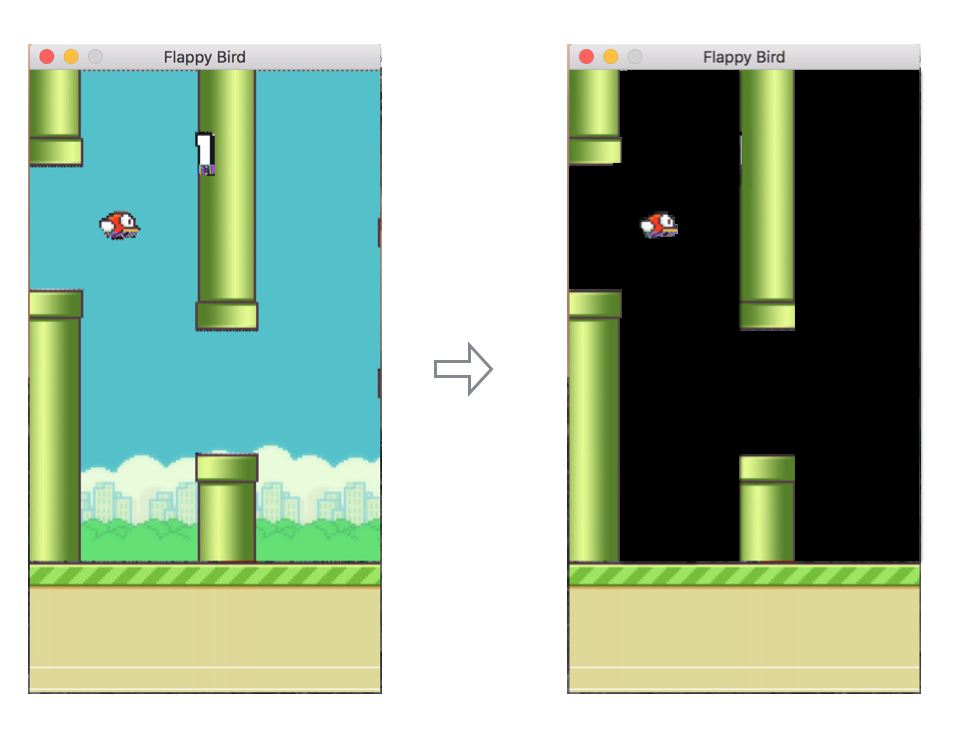
\includegraphics[width=0.9\textwidth]{Pic/preprocess}
\end{figure}

\textbf{Network Architecture}

I first preprocessed the game screens with following steps:

\begin{enumerate}
\itemsep1pt\parskip0pt\parsep0pt
\item
  Convert image to grayscale
\item
  Resize image to 80x80
\item
  Stack last 4 frames to produce an $80\times 80\times 4$ input array for network
\end{enumerate}

The architecture of the network is shown in the figure below. The first
layer convolves the input image with an $8\times 8\times 4\times 32$ kernel at a stride size
of 4. The output is then put through a $2\times 2$ max pooling layer. The second
layer convolves with a $4\times 4\times 32\times 64$ kernel at a stride of 2. We then max
pool again. The third layer convolves with a $3\times 3\times 64\times 64$ kernel at a
stride of 1. We then max pool one more time. The last hidden layer consists of 256 fully connected ReLU nodes.
\begin{figure}[ht]
\centering
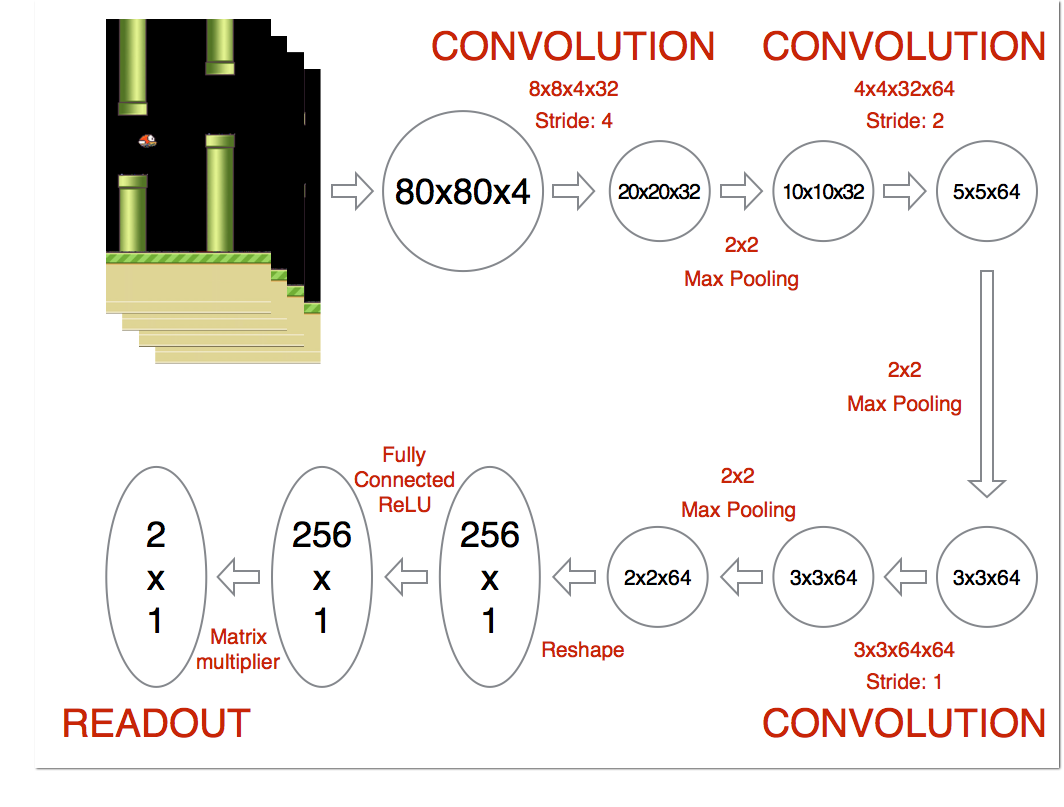
\includegraphics[width=16cm]{Pic/network}
\end{figure}

The final output layer has the same dimensionality as the number of valid actions which can be performed in the game, where the 0th index always corresponds to doing nothing. The values at this output layer
represent the $Q$ function given the input state for each valid action. At each time step, the network performs whichever action corresponds to the highest $Q$ value using a $\epsilon$ greedy policy.

\textbf{Training}

At first, I initialize all weight matrices randomly using a normal distribution with a standard deviation of 0.01, then set the replay memory with a max size of 500,00 experiences.

I start training by choosing actions uniformly at random for the first 10,000 time steps, without updating the network weights. This allows the
system to populate the replay memory before training begins.

I linearly anneal $\epsilon$from 0.1 to 0.0001 over the course of the next 3000,000 frames. The reason why I set it this way is that agent can choose an action every 0.03s (FPS=30) in our game, high $\epsilon$ will make it \textbf{flap} too much and thus keeps itself at the top of the game screen and finally bump the pipe in a clumsy way. This condition will make Q function converge relatively slow since it only start to look other conditions when $\epsilon$ is low. However, in other games, initialize $\epsilon$ to 1 is more reasonable.

During training time, at each time step, the network samples minibatches of size 32 from the replay memory to train on, and performs a gradient step on the loss function described above using the Adam optimization
algorithm with a learning rate of 0.000001. After annealing finishes, the network continues to train indefinitely, with $\epsilon$ fixed at 0.001.

\section{Tasks}
\begin{enumerate}
	\item Please implement a DQN to play the Flappy Bird game.
	\item You can refer to the codes in \url{https://github.com/yenchenlin/DeepLearningFlappyBird}
	\item Please submit a file named \texttt{E16\_YourNumber.zip}, which should includes the code files and the result pictures, and send it to \texttt{ai\_2018@foxmail.com}
\end{enumerate}
\section{Codes and Results}




\end{document} 
%%% Local Variables:
%%% mode: latex
%%% TeX-master: t
%%% End:
